%%%%%%%%%%%%%%%%%%%%%%%%%%%%%%%%%%%%%%%%%
% Ay 190 - WS2
% Written by Chatarin Wong-u-railertkun
%%%%%%%%%%%%%%%%%%%%%%%%%%%%%%%%%%%%%%%%%

%----------------------------------------------------------------------------------------
%	PACKAGES AND OTHER DOCUMENT CONFIGURATIONS
%----------------------------------------------------------------------------------------

\documentclass[11pt,letterpaper]{article}

% Load some basic packages that are useful to have
% and that should be part of any LaTeX installation.
%

\usepackage{graphicx}     % be able to include figures

\usepackage{xcolor}         % get nice colors

% change default font to Palatino (looks nicer!)
\usepackage[latin1]{inputenc}
\usepackage{mathpazo}
\usepackage[T1]{fontenc}

% load some useful math symbols/fonts
\usepackage{latexsym,amsfonts,amsmath,amssymb}
\usepackage{subcaption}

% comfort package to easily set margins
\usepackage[top=1in, bottom=1in, left=1in, right=1in]{geometry}

% control some spacings
%
% spacing after a paragraph
\setlength{\parskip}{.15cm}
% indentation at the top of a new paragraph
\setlength{\parindent}{0.0cm}

\usepackage{courier}


%----------------------------------------------------------------------------------------
%	TITLE
%----------------------------------------------------------------------------------------

\begin{document}

\begin{center}
\Large
Ay190 -- Worksheet 10 - BVP \\    %%%%%% DON'T FORGET TO CHANGE THE WORK SHEET NUMBER
Chatarin (Mee) Wong-u-railertkun\\
Date: \today
\end{center}

\section{Shooting Method}

\subsection{Forward Euler}

With FE method and number of points = 10, we compare the result. Even though values at the boundary points match pretty well, our result doesn't do very well at other points.

\begin{figure}[h!]
	\centering
	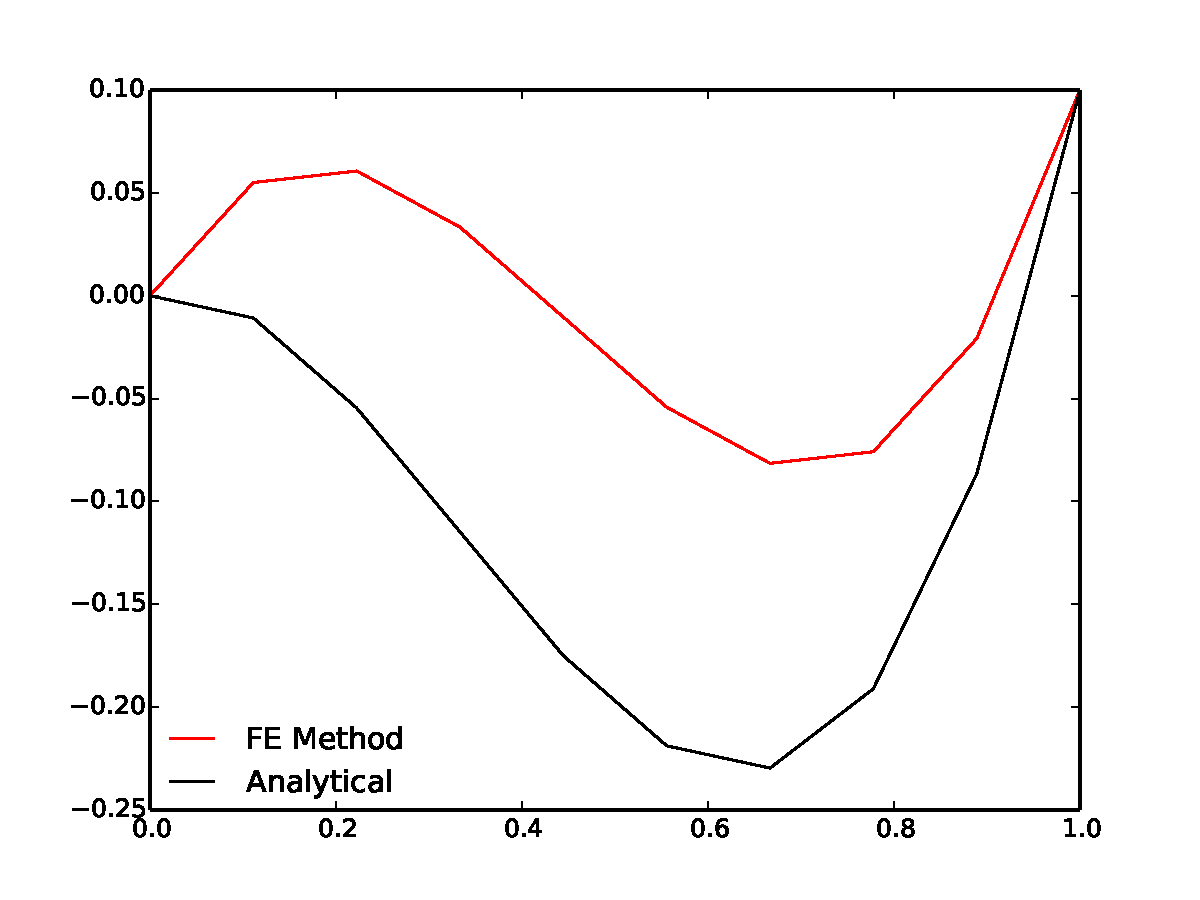
\includegraphics[width=0.5\textwidth]{FEmethod}
	\caption{Comparing result from FE with the analytical solution with number of points = 10}
	\label{fig:FEmethod}
\end{figure}

\subsection{RK2}

With RK2 method and number of points = 10, our result is so close to the analytical answer that, if plot together, it's hard to distinguish. Thus, in figure \ref{fig:RK2method}, I plot the error at each point in x. The magnitude of error is around $10^{-16}$.

\begin{figure}[h!]
	\centering
	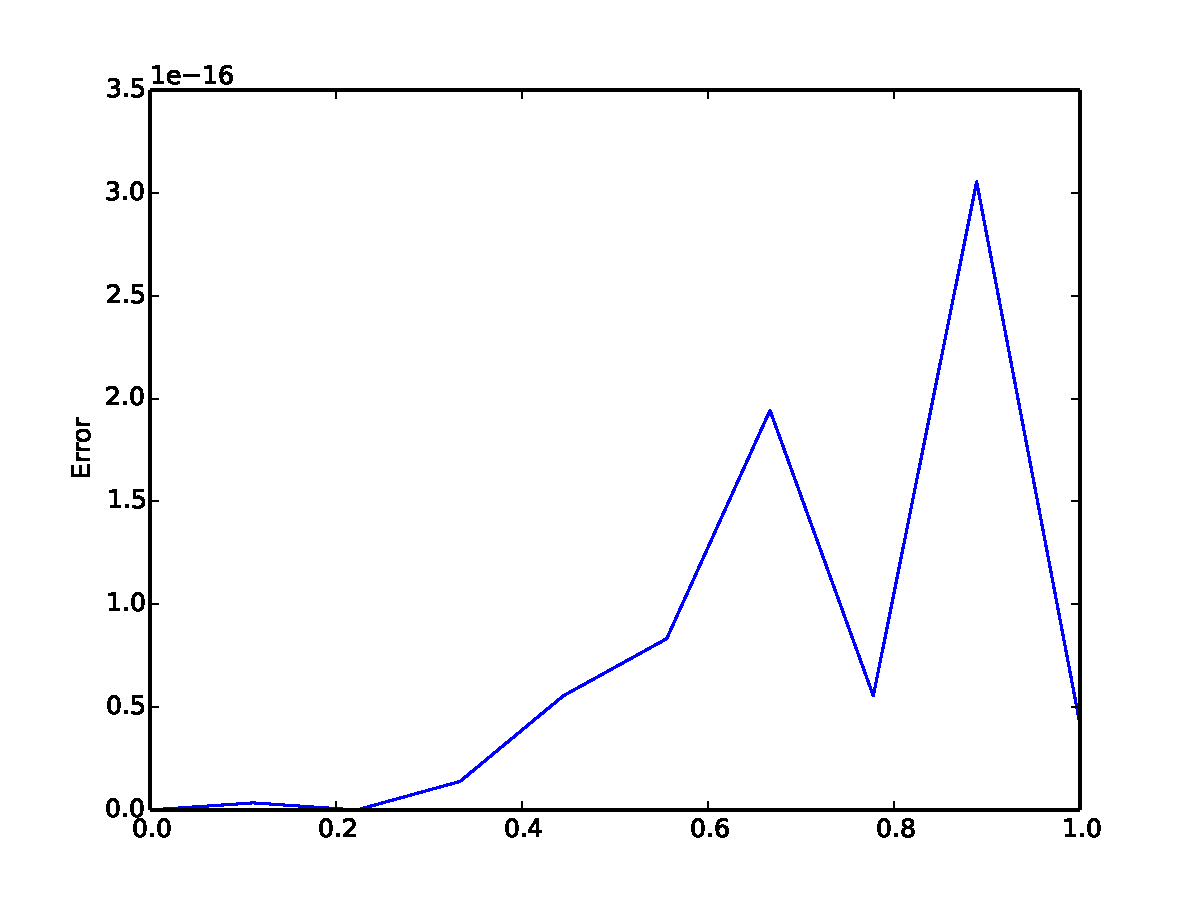
\includegraphics[width=0.5\textwidth]{RK2method}
	\caption{Showing error between result from RK2 and the analytical answer.}
	\label{fig:RK2method}
\end{figure}

\newpage
\subsection{Convergence Plot}
We can see that the error for FE drops as the expected rate. However, the error for RK2 remains pretty flat.

\begin{figure}[h!]
	\centering
	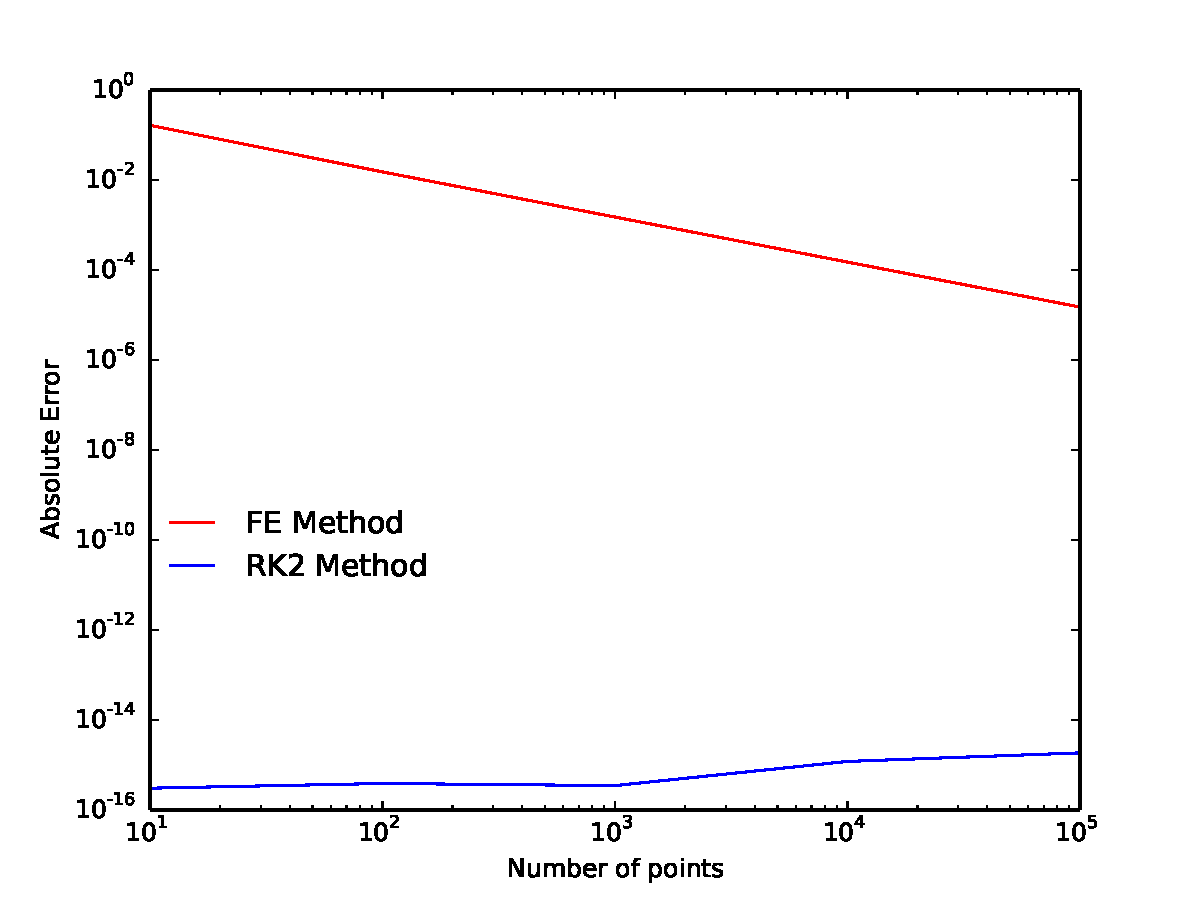
\includegraphics[width=0.5\textwidth]{ConvergePlot}
	\caption{Convergence of two methods}
	\label{fig:ConvergePlot}
\end{figure}
	
\end{document}

